\chapter{Money management}
\label{ch:money-management}

\section{Evoluzione del dimensionamento}
\label{sec:mm-evoluzione}

Il dimensionamento della posizione è, per una strategia short volatility,
tanto importante quanto la selezione dell'opzione, perché determina
l'entità del rischio sopportato a parità di segnale. L'approccio adottato è
il risultato di una progressione in tre stadi. Il primo stadio, un contratto
fisso per trade, è problematico perché il rischio per trade oscilla con il
vega dell'opzione selezionata: due trade con lo stesso numero di contratti
possono comportare esposizioni alla volatilità molto diverse. Il secondo
stadio, un obiettivo di vega fisso (pari a 50), normalizza il rischio per
trade rendendolo indipendente dallo strumento, ma non si adatta al capitale:
dopo una serie di perdite o di guadagni, l'esposizione resta la stessa in
termini assoluti. Il terzo stadio, adottato nella tesi, lega l'obiettivo di
vega al capitale corrente.

La formula del dimensionamento \emph{capital-based} è la seguente:
%
\begin{equation}
\text{vega\_target} = \frac{\text{equity} \times \text{risk\_per\_trade}}
{\text{worst\_loss\_per\_vega} \times \text{buffer}},
\label{eq:sizing}
\end{equation}
%
dove \texttt{worst\_loss\_per\_vega} è calibrato sul peggior trade
in-sample (una perdita di 2.746 dollari su 50 vega, ossia 54,93 dollari di
perdita per unità di vega) e \texttt{buffer} è un moltiplicatore prudenziale
sul worst case. L'obiettivo di vega si ricalcola a ogni trade: cresce con il
capitale, realizzando il compounding, e si riduce dopo le perdite,
attenuando automaticamente l'esposizione nei drawdown.

Un aspetto metodologico va chiarito. Le diverse configurazioni di
dimensionamento sono ottenute per riscalatura a posteriori: i trade
selezionati (date di ingresso e di uscita, strumenti) sono identici in tutte
le configurazioni, e cambia soltanto la dimensione in dollari della
posizione. Ne consegue che lo Sharpe ratio è invariante rispetto alla
configurazione, essendo un rapporto tra rendimento medio e deviazione
standard: il dimensionamento sposta la scala di rendimento e drawdown, non
la loro proporzione.

\section{Le tre configurazioni di rischio}
\label{sec:mm-configurazioni}

La Tabella~\ref{tab:configurazioni-rischio} presenta tre configurazioni,
corrispondenti a diversi appetiti per il rischio. Il parametro
\texttt{risk\_per\_trade} passa dall'1\% al 3\% del capitale, mentre il
buffer prudenziale si riduce da 2,0 a 1,0, cosicché la configurazione
conservativa è doppiamente cauta (meno rischio per trade e buffer maggiore)
e quella aggressiva doppiamente incisiva.

\begin{table}[H]
\centering
\caption{Le tre configurazioni di rischio. Lo Sharpe ratio è invariante
rispetto al dimensionamento; il trade-off è esclusivamente tra rendimento e
drawdown.}
\label{tab:configurazioni-rischio}
\small
\setlength{\tabcolsep}{4pt}
\begin{tabular}{lcccccccc}
\toprule
\textbf{Config.} & \textbf{Risk} & \textbf{Buffer} & \makecell{\textbf{Vega}\\\textbf{in.}} & \textbf{Ret IS} & \textbf{DD IS} & \makecell{\textbf{Ret}\\\textbf{OOS}} & \makecell{\textbf{DD}\\\textbf{OOS}} & \makecell{\textbf{Sharpe}\\\textbf{IS/OOS}} \\
\midrule
Conservativa & 1\% & 2,0$\times$ & 9,1  & $+6{,}9\%$  & $-3{,}9\%$  & $+2{,}6\%$  & $-0{,}9\%$ & 1,75/1,52 \\
Moderata     & 2\% & 1,5$\times$ & 24,3 & $+19{,}3\%$ & $-10{,}3\%$ & $+7{,}0\%$  & $-2{,}3\%$ & 1,75/1,52 \\
Aggressiva   & 3\% & 1,0$\times$ & 54,6 & $+47{,}8\%$ & $-22{,}6\%$ & $+16{,}1\%$ & $-5{,}1\%$ & 1,75/1,52 \\
\bottomrule
\end{tabular}
\end{table}

L'invarianza dello Sharpe ha un'implicazione importante: la scelta della
configurazione non è una scelta di qualità della strategia, ma di
tolleranza al drawdown. Un investitore che accetti un drawdown atteso fino
al $-22{,}6\%$ in-sample può adottare la configurazione aggressiva e mirare
a un rendimento del $+47{,}8\%$; uno più prudente si accontenterà del
$+6{,}9\%$ della configurazione conservativa con un drawdown contenuto entro
il $-3{,}9\%$. La strategia sottostante è la medesima. La configurazione
aggressiva, con vega iniziale di 54,6, è peraltro quasi identica al vega
fisso pari a 50 dello stadio precedente: il vantaggio del dimensionamento
capital-based non è un'esposizione diversa, ma la sua adattività automatica
al capitale.

Non sono stati adottati altri metodi di dimensionamento per ragioni
specifiche. Il criterio di Kelly pieno, come discusso nella sezione
seguente, richiede stime di parametri troppo rumorose su 35 trade. Il
\emph{vol targeting} ha senso per portafogli multi-posizione con
correlazioni variabili, non per una strategia a posizione singola. Lo
\emph{scaling} sul drawdown è già incorporato implicitamente nel
dimensionamento capital-based, poiché un calo del capitale riduce
automaticamente l'obiettivo di vega.

\section{Half-Kelly come sanity check}
\label{sec:mm-kelly}

Il criterio di \citet{kelly1956new} è stato calcolato non come metodo di
dimensionamento, ma come verifica di coerenza della prudenza delle
configurazioni adottate. A partire dai 35 trade in-sample, con un win rate
del 65,7\% e un rapporto di payoff di 2,57 (guadagno medio 1,76\% contro
perdita media 0,69\%), la frazione di Kelly risulta
%
\begin{equation}
f^{*} = 0{,}657 - \frac{1 - 0{,}657}{2{,}57} = 52{,}4\%,
\end{equation}
%
e la sua metà (Half-Kelly), la frazione prudenziale di uso comune, vale il
26,2\%, corrispondente a un obiettivo di vega di circa 477. Il confronto con
le tre configurazioni è netto: la conservativa impiega il 2\% del
Half-Kelly, la moderata il 5\% e l'aggressiva l'11\%. Anche la
configurazione più incisiva opera dunque a poco più di un decimo del
Half-Kelly.

Questa estrema prudenza è intenzionale e proporzionata all'incertezza.
Trentacinque trade sono pochi per stimare con precisione i parametri di
Kelly, la cui sensibilità agli errori di input è nota. Il criterio assume
inoltre distribuzioni stazionarie e indipendenza tra i trade, ipotesi
fragili per una strategia esposta a salti e a esplosioni di volatilità, come
mostra il worst case in-sample (una perdita non realizzata del $-15{,}5\%$).
Nella prassi, del resto, nessun operatore istituzionale opera oltre il
10--15\% del Kelly. Il sanity check conferma quindi che le configurazioni
non sono irragionevolmente conservative, ma prudenti in misura commisurata
all'incertezza dei parametri.

\section{Margini Deribit e soglia di rovina}
\label{sec:mm-margini}

Il dimensionamento deve tenere conto dei margini richiesti dall'exchange. La
Tabella~\ref{tab:margini} riporta il margine iniziale, calcolato secondo la
formula Standard Margin di Deribit per opzioni corte, sui 35 trade
in-sample e per ciascuna configurazione.

\begin{table}[H]
\centering
\caption{Margine iniziale (Standard Margin Deribit) calcolato sui 35 trade
in-sample, per configurazione.}
\label{tab:margini}
\begin{tabular}{lccc}
\toprule
\textbf{Configurazione} & \textbf{IM medio} & \textbf{IM worst-case} & \textbf{Capitale min (1,5$\times$)} \\
\midrule
Conservativa (vega 9,1)  & \$1.672  & \$6.205  & \$9.308 \\
Moderata (vega 24,3)     & \$4.465  & \$16.570 & \$24.855 \\
Aggressiva (vega 54,6)   & \$10.033 & \$37.232 & \$55.847 \\
\bottomrule
\end{tabular}
\end{table}

Ne discende una soglia di rovina operativa di circa 10.000 dollari: al di
sotto di questo livello non è possibile aprire neppure un singolo trade
nella configurazione più conservativa mantenendo un buffer di margine
adeguato. Con il dimensionamento capital-based questa soglia vale per tutte
le configurazioni, poiché l'esposizione si adatta automaticamente al
capitale disponibile. Va notato che il margine worst-case include un trade
con delta pari a 0,75 all'ingresso: il filtro $|\Delta| \le 0{,}50$ è
applicato alla data del segnale, ma il delta si muove tra segnale ed
esecuzione (il trade in questione aveva delta $-0{,}495$ al segnale e
$-0{,}755$ all'ingresso, per effetto di un movimento overnight di Bitcoin).
Si tratta di uno scivolamento realistico e non evitabile.

\section{Rischio di rovina: simulazione Monte Carlo}
\label{sec:mm-montecarlo}

Il drawdown realizzato nel backtest è una singola traiettoria: per valutare
il rischio in modo prospettico occorre chiedersi quanto avrebbe potuto
essere diverso, a parità di caratteristiche statistiche della strategia. A
questo scopo è stata condotta una simulazione Monte Carlo basata sul
\emph{circular block bootstrap} dei rendimenti giornalieri mark-to-market
del periodo in-sample: per ciascuna configurazione, 10.000 percorsi della
stessa lunghezza del periodo in-sample (845 giorni) sono generati
ricampionando blocchi contigui di 20 giorni di rendimenti effettivi. Il
ricampionamento a blocchi, anziché per singole osservazioni, preserva il
raggruppamento temporale delle perdite (i giorni negativi tendono a
concentrarsi nei periodi di stress, come il crash del 2022), che è la
caratteristica che rende profondi i drawdown; i risultati sono robusti alla
scelta della lunghezza del blocco (la mediana varia di meno di un punto
percentuale tra blocchi di 5 e di 40 giorni). Accanto allo scenario base è
stato simulato uno scenario di stress dichiarato, in cui ogni rendimento
giornaliero negativo è amplificato del 50\% prima del ricampionamento: uno
scenario severo per costruzione, poiché il peggioramento si applica
sistematicamente per l'intero orizzonte. La soglia di rovina è fissata a
10.000 dollari (\S\ref{sec:mm-margini}).

\begin{table}[H]
\centering
\caption{Distribuzione del max drawdown dalla simulazione Monte Carlo
(block bootstrap dei rendimenti giornalieri MTM in-sample, 10.000 percorsi
di 845 giorni). La colonna ``realizzato'' riporta il drawdown
effettivamente osservato nel backtest: la sua vicinanza alla mediana
simulata conferma la coerenza del modello. P(rovina): frazione di percorsi
che raggiunge la soglia di 10.000 dollari.}
\label{tab:montecarlo-dd}
\footnotesize
\setlength{\tabcolsep}{3pt}
\begin{tabular}{lccccccc}
\toprule
 & & \multicolumn{3}{c}{\textbf{Scenario base}} & \multicolumn{2}{c}{\textbf{Stress ($\times$1,5)}} & \\
\cmidrule(lr){3-5}\cmidrule(lr){6-7}
\textbf{Configurazione} & \textbf{Realizz.} & \textbf{Mediana} & \textbf{P95} & \textbf{P99} & \textbf{Mediana} & \textbf{P95} & \textbf{P(rovina)} \\
\midrule
Conservativa (1\%) & $-3{,}9\%$  & $-3{,}7\%$  & $-5{,}9\%$  & $-7{,}5\%$  & $-18{,}0\%$ & $-25{,}0\%$ & 0{,}00\% \\
Moderata (2\%)     & $-10{,}3\%$ & $-9{,}7\%$  & $-15{,}1\%$ & $-18{,}8\%$ & $-41{,}6\%$ & $-54{,}6\%$ & 0{,}00\% \\
Aggressiva (3\%)   & $-22{,}6\%$ & $-21{,}4\%$ & $-31{,}9\%$ & $-38{,}7\%$ & $-71{,}4\%$ & $-83{,}9\%$ & 0{,}00\% \\
\bottomrule
\end{tabular}
\end{table}

\begin{figure}[H]
\centering
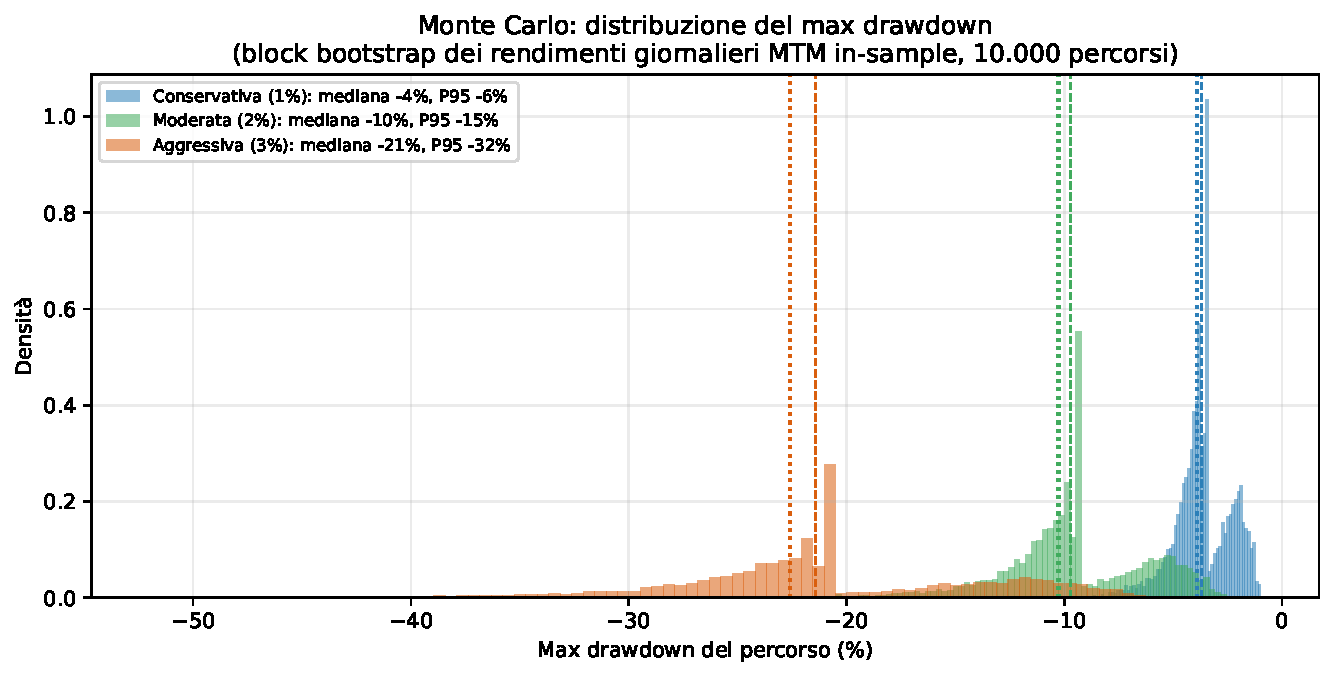
\includegraphics[width=\textwidth]{figures/fig_mc_drawdown.pdf}
\caption{Distribuzione del max drawdown nei 10.000 percorsi simulati
(scenario base), per configurazione. Le linee tratteggiate indicano le
mediane; le linee puntinate il drawdown realizzato nel backtest, che in
tutte le configurazioni cade in prossimità della mediana simulata.}
\label{fig:mc-drawdown}
\end{figure}

Tre osservazioni. Primo, la validazione del modello: il drawdown realizzato
nel backtest cade in prossimità della mediana simulata per tutte le
configurazioni ($-3{,}9\%$ contro $-3{,}7\%$; $-10{,}3\%$ contro
$-9{,}7\%$; $-22{,}6\%$ contro $-21{,}4\%$). L'esperienza storica è dunque
una realizzazione tipica della distribuzione, non un caso fortunato, e i
percentili estremi (P95 e P99) quantificano quanto peggio sarebbe potuta
andare a parità di strategia: circa una volta e mezza il drawdown storico
al 95\textsuperscript{o} percentile e quasi il doppio al
99\textsuperscript{o}.

Secondo, il rischio di rovina è nullo in tutte le configurazioni nello
scenario base: nessuno dei 10.000 percorsi si avvicina alla soglia (il
percorso peggiore della configurazione aggressiva perde circa il 39\%,
contro il 90\% necessario per la rovina). Anche nello scenario di stress la
probabilità di rovina resta nulla per le configurazioni conservativa e
moderata, e trascurabile (0,23\%) per l'aggressiva. La rovina, in senso
proprio, non è il rischio rilevante di questa strategia.

Terzo, il vincolo operativo è il drawdown, e lo scenario di stress rende
esplicito il trade-off tra le configurazioni: se il futuro fosse
sistematicamente peggiore del passato (ogni giornata negativa il 50\% più
severa, per anni), la configurazione moderata arriverebbe a un drawdown
mediano del $-41{,}6\%$ e l'aggressiva del $-71{,}4\%$, mentre la
conservativa si fermerebbe al $-18{,}0\%$. La scelta della configurazione
dipende dunque dalla tolleranza al drawdown nello scenario avverso, non dal
rischio di rovina, che resta remoto ovunque.

La Figura~\ref{fig:mc-paths} chiude l'analisi mostrando la stessa
simulazione dal punto di vista dell'evoluzione temporale: un campione dei
percorsi di equity simulati, con la banda tra il 5\textsuperscript{o} e il
95\textsuperscript{o} percentile, la mediana e, sovrapposta, la curva
realizzata dal backtest. Il grafico rende visiva la validazione del
modello: la curva realizzata attraversa la banda simulata restando prossima
alla mediana per l'intero orizzonte, in tutte le configurazioni. La soglia
di rovina (10\% dell'equity iniziale) giace molto al di sotto
dell'intervallo mostrato: anche il percorso peggiore dell'intera
simulazione non vi si avvicina.

\begin{figure}[H]
\centering
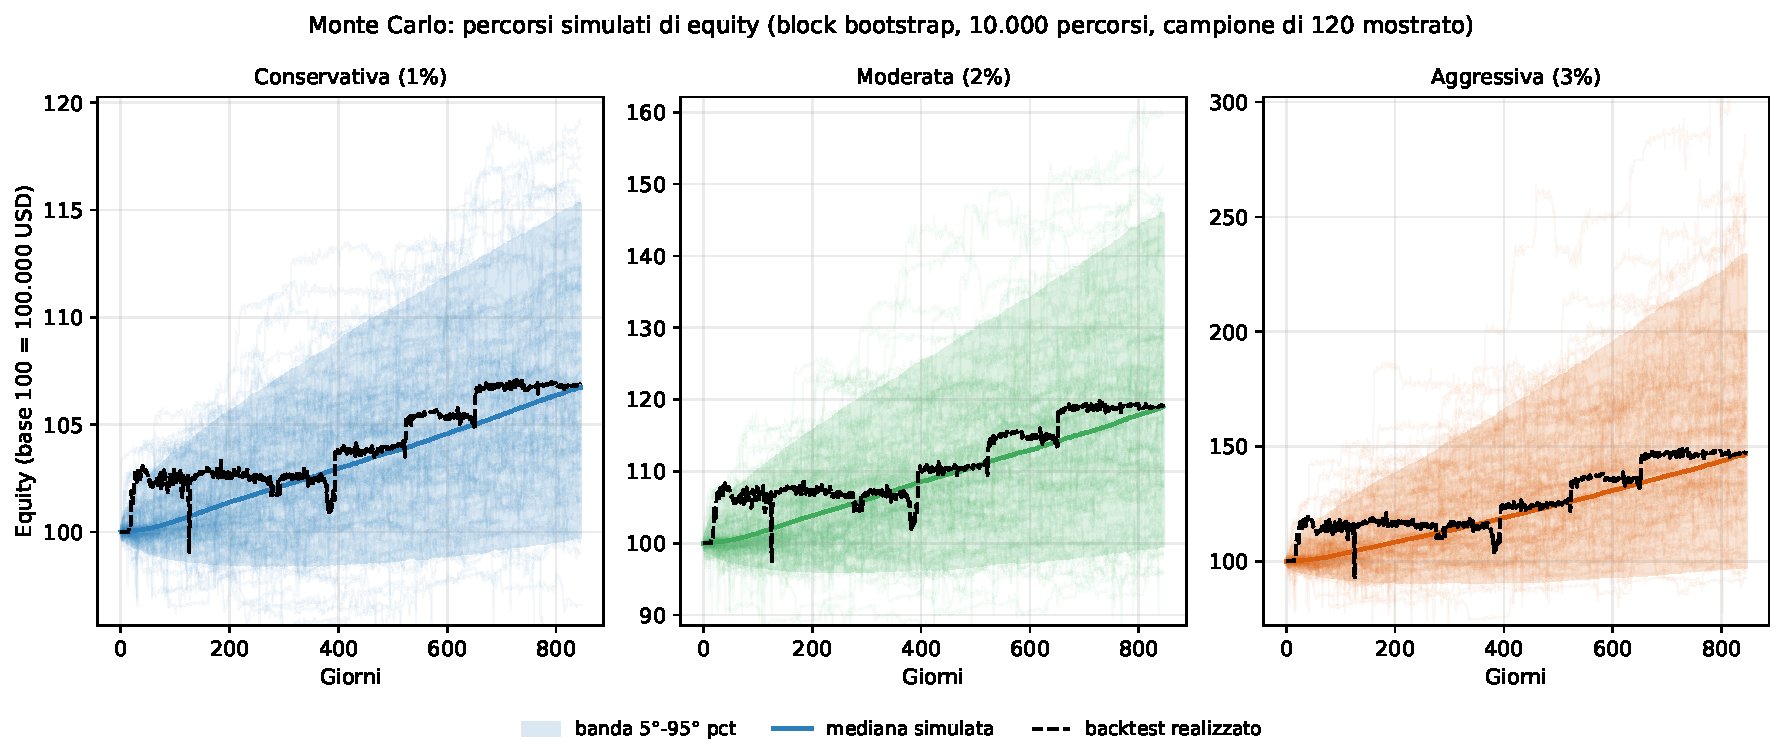
\includegraphics[width=\textwidth]{figures/fig_mc_paths.pdf}
\caption{Percorsi simulati di equity (scenario base): campione di 120
percorsi, banda 5\textsuperscript{o}--95\textsuperscript{o} percentile,
mediana simulata e curva realizzata dal backtest (tratteggiata). La curva
realizzata resta prossima alla mediana simulata in tutte le configurazioni;
la soglia di rovina (10\% dell'equity iniziale) è fuori scala, molto al di
sotto dell'intervallo mostrato.}
\label{fig:mc-paths}
\end{figure}
